
\lhead[\chaptername~\thechapter]{\rightmark}

\rhead[\leftmark]{}

\lfoot[\thepage]{}

\cfoot{}

\rfoot[]{\thepage}

\chapter{Results}

The most relevant results of the analysis are shown and organized
in this chapter. As a first step, the number of states of the model
was decided (Analysis I). Then, the number of parameters that have
switching effects in the model was determined (Analysis II). A model
selection was performed for Analysis I and Analysis II in order to
find the most appropriate model for each given dataset. An analysis
of residuals was carried out as a means to validate the models. The
results are shown in a later section. Next, the results of a non-parametric
analysis are presented, and a comparison between the results of Markov
switching model analysis and the results of non-parametric analysis
are illustrated. The last two sections report the results of a state
prediction of the new observations in each dataset, and an evaluation
of the predicting function using a simulated data. 

\section{Analysis I: Number of States \label{sec:States}}

To estimate the set of necessary parameters, the \emph{MSwM}\footnote{https://cran.r-project.org/web/packages/MSwM/index.html}
package in R was used. More details about the package can be found
in \ref{sec:MSwM-Package}. A complete linear Markov switching model
in this thesis framework is defined as

\begin{align}
y_{t}= & \beta_{intercept,S_{t}}+\beta_{RrcConnectionSetupComplete,S_{t}}X_{RrcConnectionSetupComplete,t}\nonumber \\
 & +\beta_{Paging,S_{t}}X_{Paging,t}+\beta_{X2HandoverRequest,S_{t}}X_{X2HandoverRequest,t}\label{eq:mswm}\\
 & +\beta_{DuProdName,S_{t}}X_{DuProdName,t}+\beta_{Fdd/Tdd,S_{t}}X_{Fdd/Tdd,t}\nonumber \\
 & +\beta_{NumCells,S_{t}}X_{NumCells,t}+\phi_{1,S_{t}}y_{t-1}+\varepsilon_{S_{t}}\nonumber 
\end{align}

The estimation was made under the assumptions of two or three states
$S_{t}\in S$, where $S={1,2,..,k}$ and $k=2$ or $3$. These two
numbers come from a hypothesis that the state of the CPU utilization
might have two states (\emph{Steady} and \emph{Degradation}, \emph{Steady}
and \emph{Improvement}, \emph{Degradation} and \emph{Improvement})
or three states (\emph{Steady}, \emph{Degradation}, and \emph{Improvement}).
During the estimation, a normality assumption was also applied to
the distribution of residuals. 

BICs from fitting the Markov switching model are shown in \ref{state-bic}.
For the software release A, the BIC suggests that the three-state
Markov switching model gives a better fit in comparison to the two-state
model. However, the models with two states for the remaining two software
releases, B and C, had lower BICs. 

\begin{table}[h]
\caption{BIC of the model with two and three states. The left column gives
the different datasets.}
\label{state-bic}
\centering{}%
\begin{tabular}{cr@{\extracolsep{0pt}.}lr@{\extracolsep{0pt}.}l}
\toprule 
\multirow{2}{*}{$\quad$Software release$\quad$} & \multicolumn{4}{c}{BIC}\tabularnewline
\cmidrule{2-5} 
 & \multicolumn{2}{c}{$k=2$} & \multicolumn{2}{c}{$k=3$}\tabularnewline
\midrule
\midrule 
A & 439&677 & 417&682\tabularnewline
B & 1,763&507 & 1,797&259\tabularnewline
C & 1,189&061 & 1,199&075\tabularnewline
\bottomrule
\end{tabular}
\end{table}


\subsection{Software release A}

Before performing the Markov switching model, a standard linear regression
model was fitted to the dataset first. It was found that a coefficient
of \emph{DuProdName} in the dataset of the software release A was
not defined because of singularity i.e., a perfect correlation between
predictor variables. Hence, \emph{DuProdName }was dropped from Equation
\ref{eq:mswm}. 

\ref{L16A_2_smo} presents that the Markov chain remained in State1
for an extensive period of time before it switched to State2. When
the chain is in State2, it stays there only a short time and then
quickly moves back to State1. There are a few switches between these
two states in \ref{L16A_2_smo}. On the other hand, it is visible
that there are more switches between states in \ref{L16A_3_smo}.
Note that State2 in the two-state model seems to be defined as State1
in the three-state model instead. Moreover, the periods of State1,
which has a rather long duration in the two-state model, now contains
several switches between states in the three-state model.

\begin{figure}[H]
\centering{}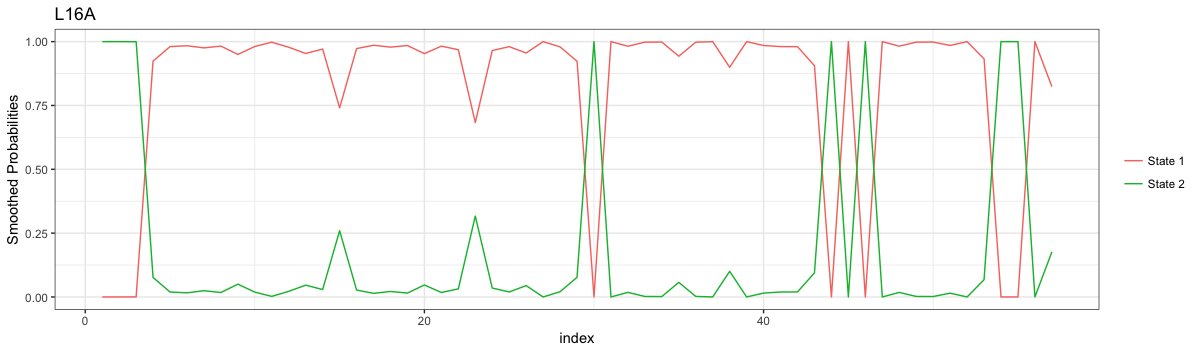
\includegraphics[scale=0.35]{picture/L16A_2_smo1}\caption{The smoothed probabilities of the software release A with two-state
model}
\label{L16A_2_smo}
\end{figure}

\begin{figure}[H]
\centering{}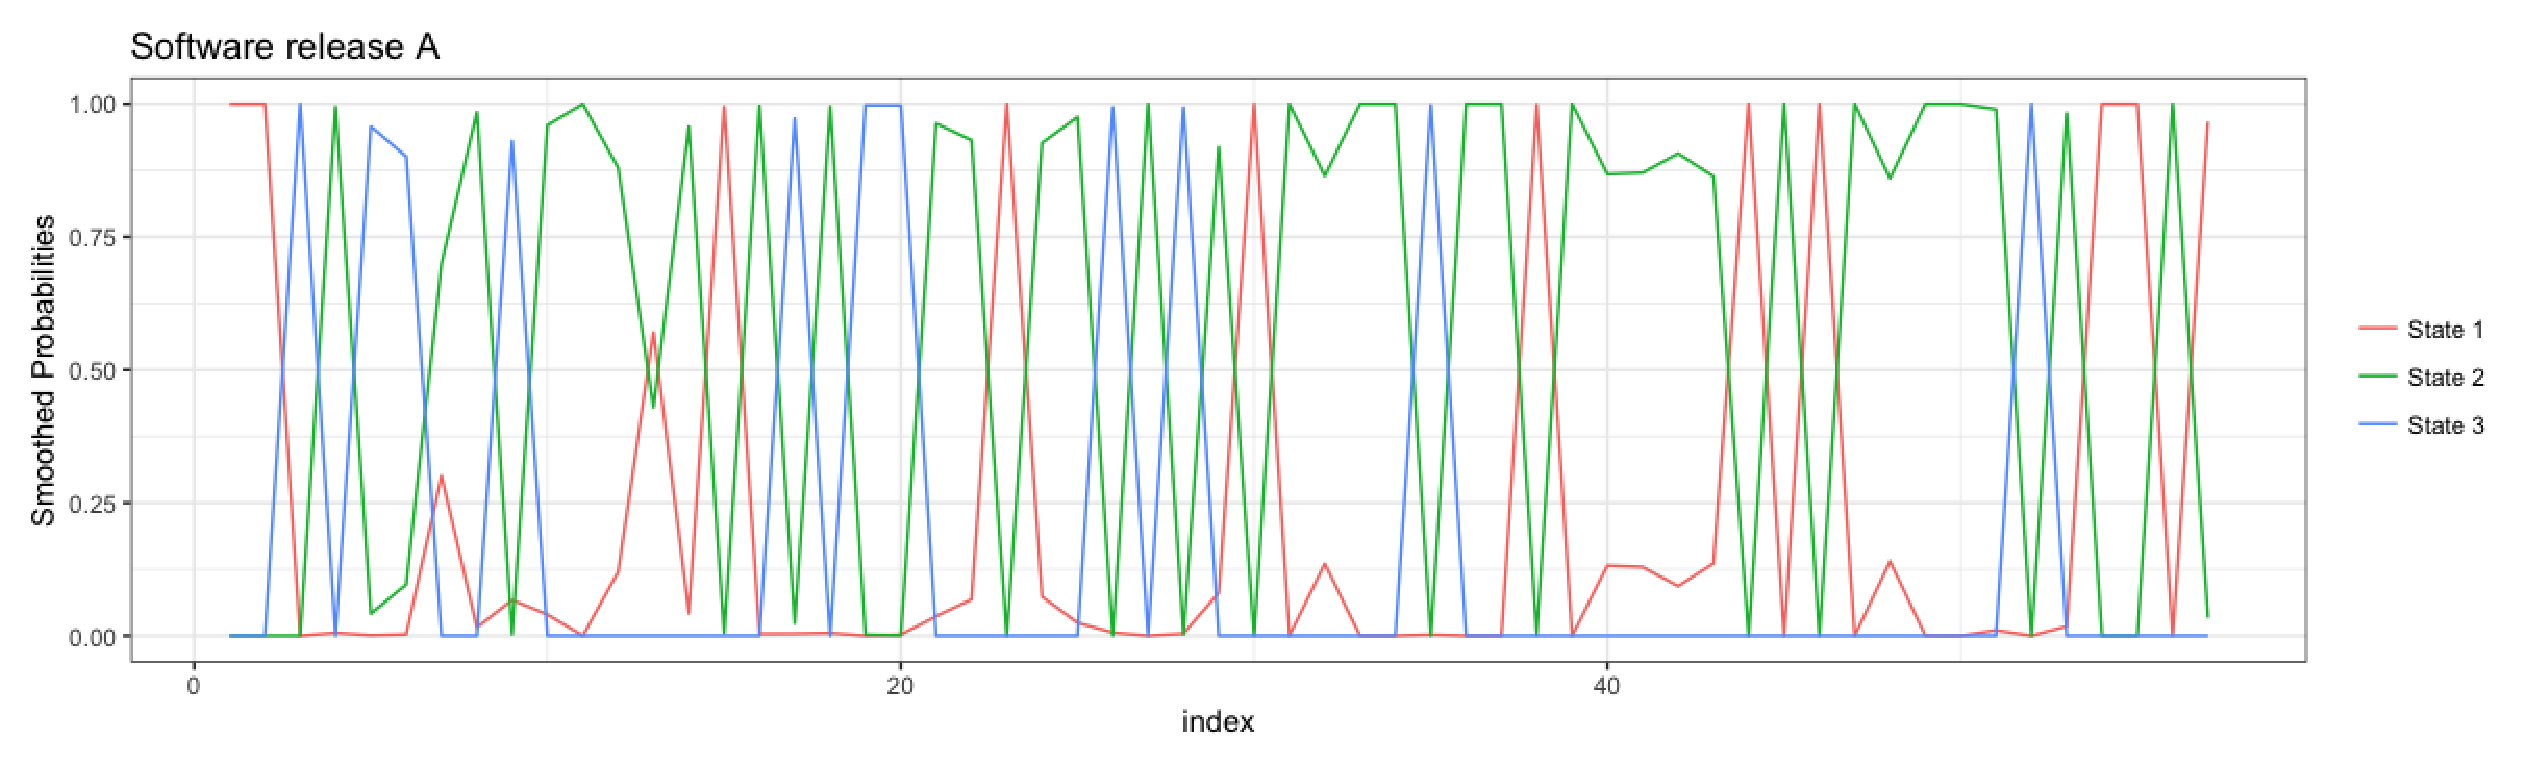
\includegraphics[scale=0.35]{picture/L16A_3_smo1}\caption{The smoothed probabilities of the software release A with three-state
model}
\label{L16A_3_smo}
\end{figure}


\subsection{Software release B}

In \ref{L16B_2_smo}, the Markov chain has several periods where it
switches back and forth between two states of the software release
B. The duration of the chain being in State2 is longer than the duration
of the chain staying in State 1. Although the chain briefly stays
in State1, it remains in this state for a few moments in the middle
of the time period (observation 91-99 and 101-114) before returning
to State2. Apparently, there are more switches between states in the
three-state model, especially in the beginning, middle, and at the
end of the period. \ref{L16B_3_smo} shows that the chain remains
in State3 over a considerable period as shown throughout observations
15-39, 42-67, and 140-170.

\begin{figure}[H]
\begin{centering}
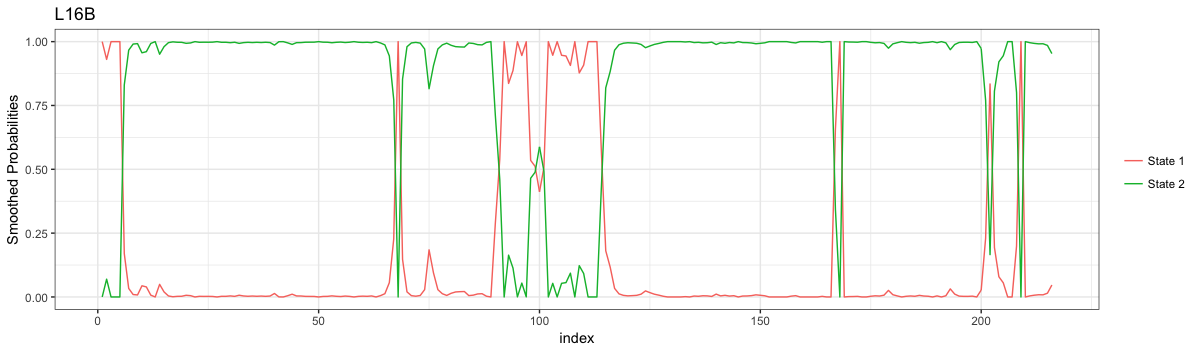
\includegraphics[scale=0.35]{picture/L16B_2_smo1}
\par\end{centering}
\caption{The smoothed probabilities of the software release B with two-state
model}
\label{L16B_2_smo}
\end{figure}

\begin{figure}[H]
\begin{centering}
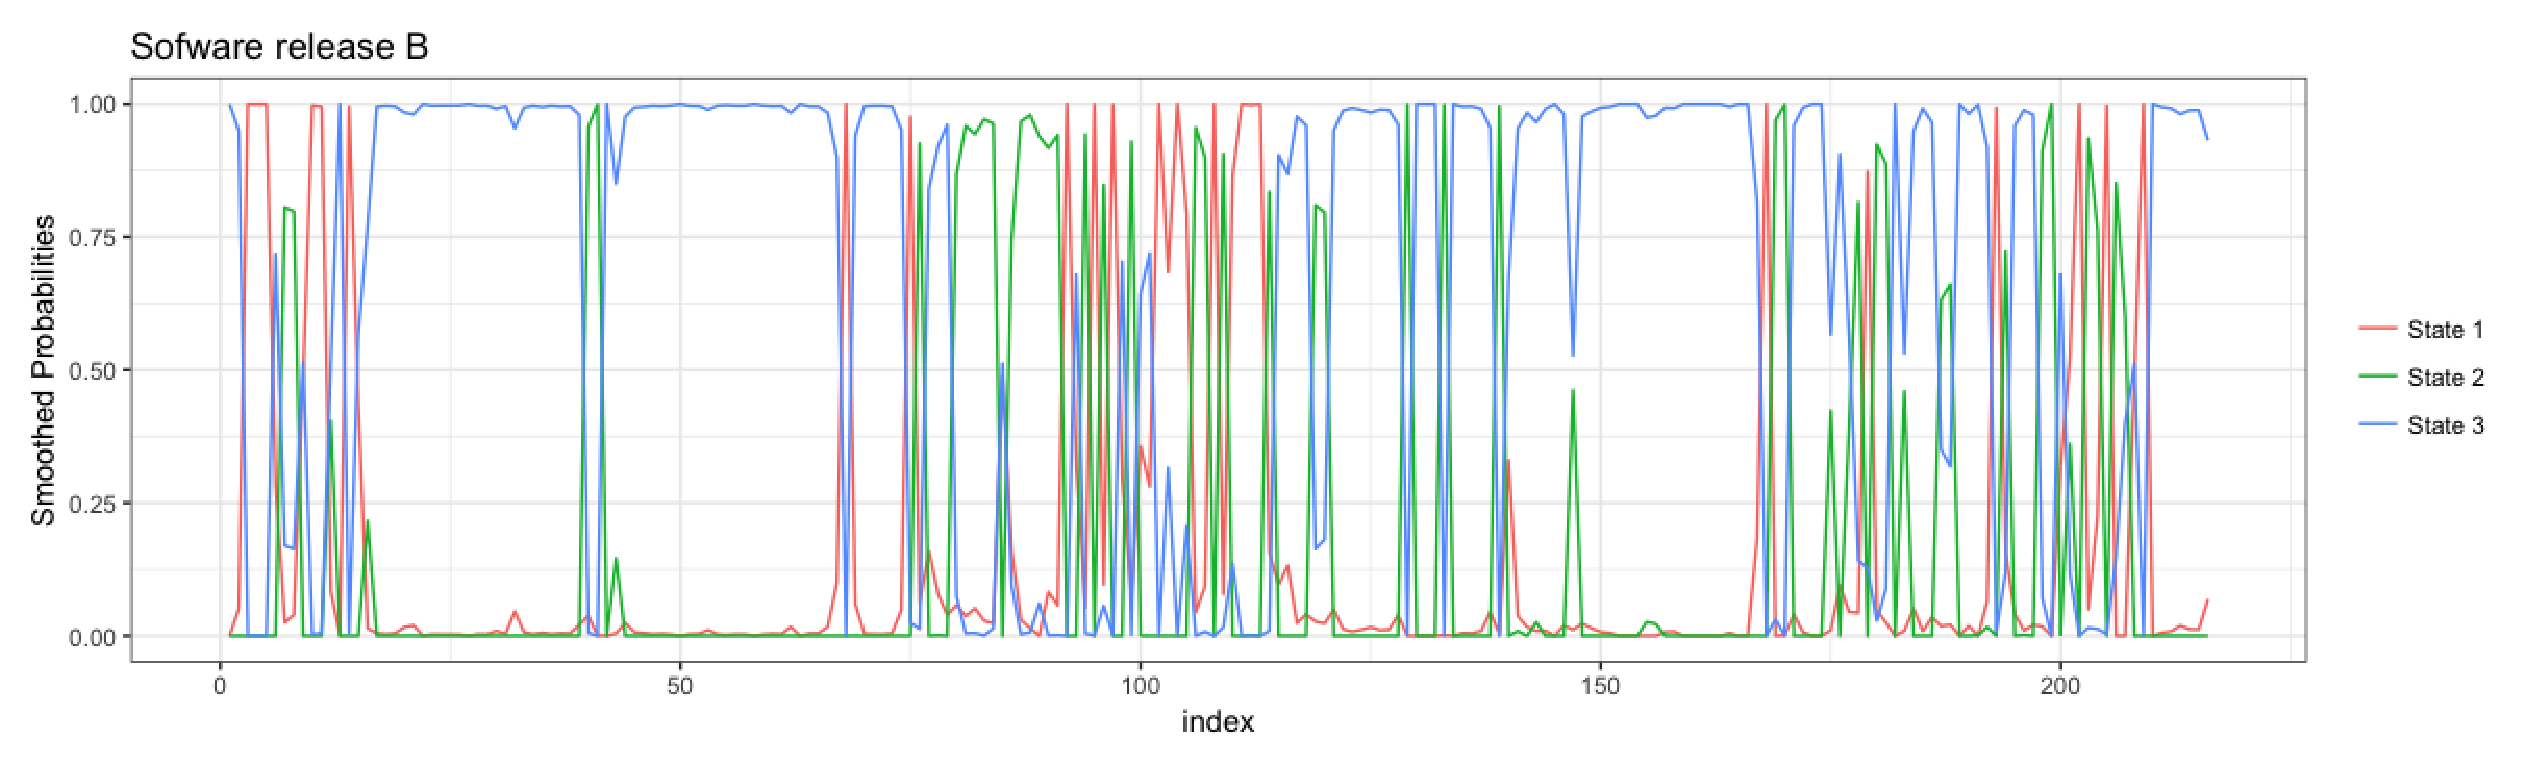
\includegraphics[scale=0.35]{picture/L16B_3_smo1}
\par\end{centering}
\caption{The smoothed probabilities of the software release B with three-state
model}
\label{L16B_3_smo}
\end{figure}

\begin{figure}[H]
\subfloat[Close-up on the observations 0-20]{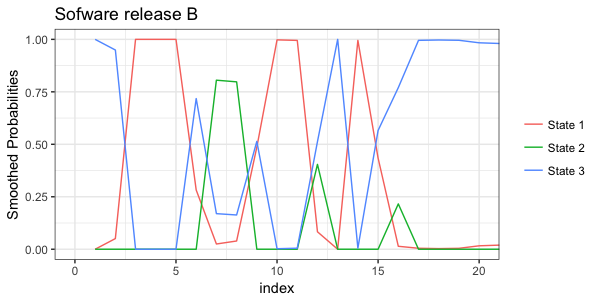
\includegraphics[scale=0.35]{picture/L16B_3_1}

}\subfloat[Close-up on the observations 75-115]{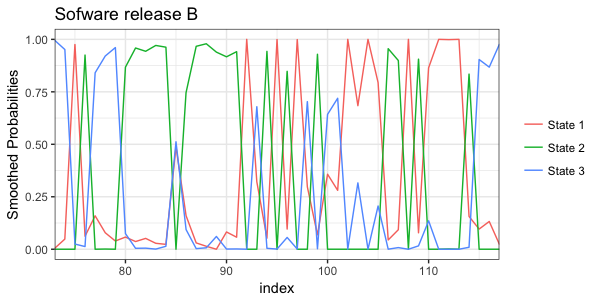
\includegraphics[scale=0.35]{picture/L16B_3_2}

}

\subfloat[Close-up on the observations 165-210]{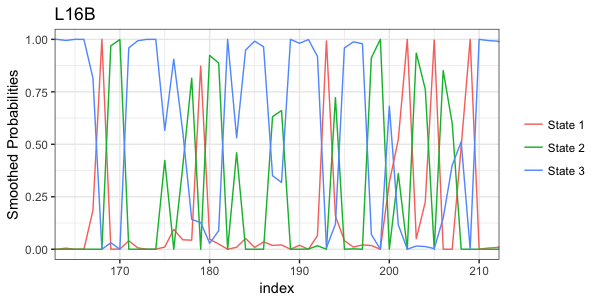
\includegraphics[scale=0.35]{picture/L16B_3_3}

}

\caption{Close-up for the smoothed probabilities of the software release B
from \ref{L16B_3_smo}}
\end{figure}


\subsection{Software release C}

There are a number of switches between states in the two-state model
of the software release C. In \ref{L17A_2_smo}, when the Markov chain
is in State1, it continues to stay in its state for a while before
leaving to State2. Furthermore, the chain stays a fairly short duration
in State2. After the chain visits State2, it instantly switches back
to State1. \ref{L17A_3_smo} presents the chain which has many switches
between State1 and State3 in the first half of the time period. The
chain for the three-state model also stays in State2 significantly
long from observation 104 to 129, which is the end of the time series.

\begin{figure}[H]
\centering{}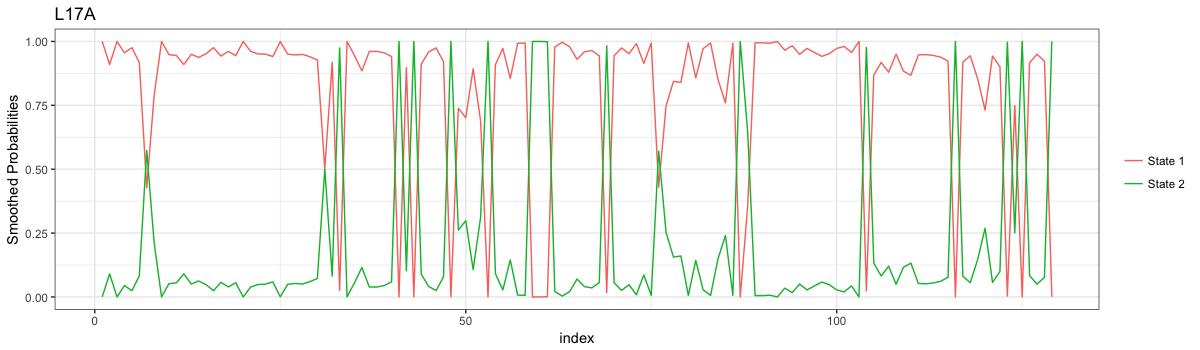
\includegraphics[scale=0.35]{picture/L17A_2_smo1}\caption{The smoothed probabilities of the software release C with two-state
model}
\label{L17A_2_smo}
\end{figure}
\begin{figure}[H]
\centering{}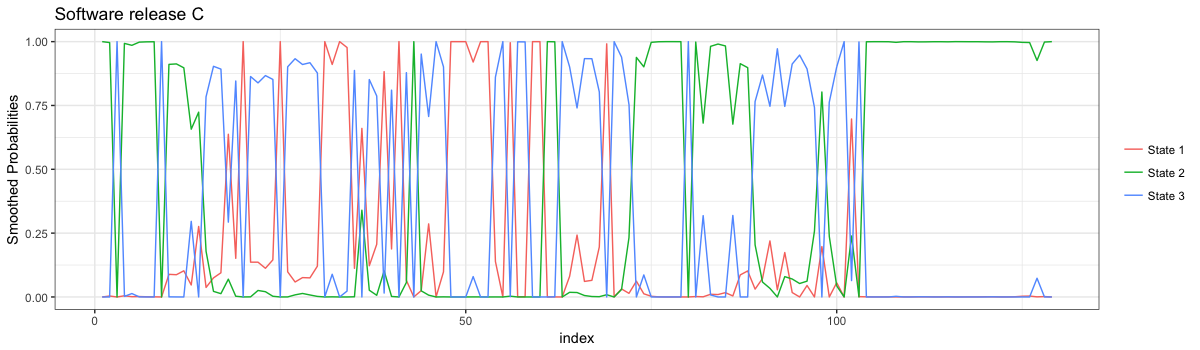
\includegraphics[scale=0.35]{picture/L17A_3_smo1}\caption{The smoothed probabilities of the software release C with three-state
model}
\label{L17A_3_smo}
\end{figure}

\begin{figure}[H]
\subfloat[Close-up on the observations 15-45]{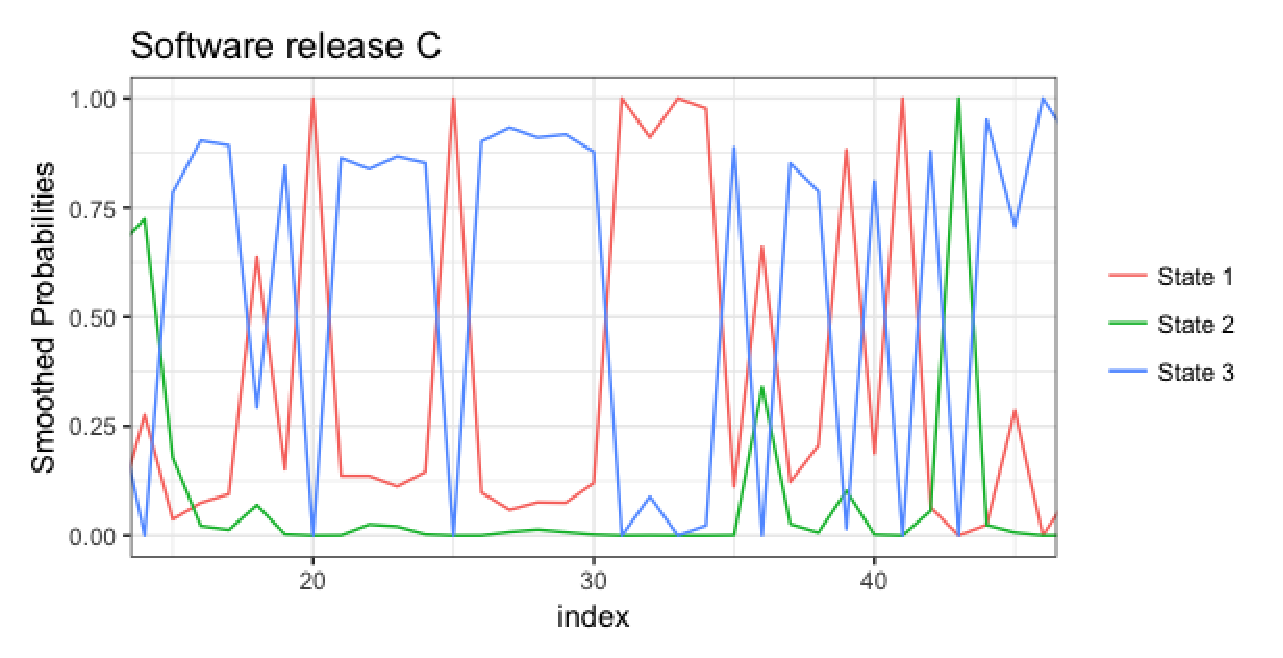
\includegraphics[scale=0.35]{picture/L17A_3_1}

}

\caption{Close-up for the smoothed probabilities of the software release C
from \ref{L17A_3_smo}}

\end{figure}

After examining the outputs from the models along with the plots,
the three-state models for each software release were further analyzed
in the thesis. More details are provided in \ref{chap:Discussion}. 

\section{Analysis II: Number of Switching coefficients \label{sec:Switching}}

In this section, the number of switching coefficients to be included
in the model were decided based on applying the Markov switching model
with the selected number of states from Analysis I i.e., three-state
Markov switching model. The fitted Markov switching models in Analysis
I were performed by assuming that every parameter in the model had
switching effects i.e., coefficients can have different values in
different periods. However, in practice, each coefficient can have
either a switching or non-switching effect. Therefore, Markov switching
models were applied to each dataset again but with a hypothesis that
the variables considered as a test environment are possible to have
non-switching effects. In this section, the structure of all the models
from all three datasets are reported in the tables. The best model
is selected for each dataset and its state specification is presented
in the plots. Further discussion and details about these chosen models
are provided in \ref{subsec:Model-selection}. It should be noted
that these three chosen models will later be used throughout this
thesis, and the model outputs are shown in \ref{chap:Output}. 

\subsection{Software release A}

For the dataset of the software release A, \emph{DuProdName} was not
included in the model fitting as explained previously. Only two variables
of the test environment were left to try whether they could have non-switching
effects or not. The result is shown in \ref{L16A_switch}. The second
model has the highest BIC and even higher than the model which have
all switching coefficients. The first model, where both \emph{Fdd/Tdd}
and \emph{NumCells} do not have switching effects, was selected to
be used with this dataset. 

\begin{table}[h]
\caption{List of the model structure of the software release A along with its
BIC. The last line is the result taken from the three-state model
in the Analysis I. The line in bold indicates the selected model.}
\label{L16A_switch}
\centering{}%
\begin{tabular}{cccc}
\toprule 
\multirow{2}{*}{Model} & \multicolumn{2}{c}{Switching effect} & \multirow{2}{*}{BIC}\tabularnewline
\cmidrule{2-3} 
 & Fdd/Tdd & NumCells & \tabularnewline
\midrule
\midrule 
\textbf{1} & \textbf{N} & \textbf{N} & \textbf{413.408}\tabularnewline
2 & N & Y & 438.371\tabularnewline
3 & Y & N & 401.232\tabularnewline
\midrule
 & Y & Y & 417.682\tabularnewline
\bottomrule
\end{tabular}
\end{table}

\ref{L16A_NN} indicates the CPU utilization of the software release
A and also shows the periods of the derived state from the model.
From the plot, State2 clearly has the longest duration without switching
state. When the chain moves to either State1 or State3, most of the
time it immediately switches to another state. However, the duration
when the chain stays in State1 is longer in the beginning and almost
at the end of the period. Another characteristic that could be observed
is that State2 switches more often to State3 rather than to State1.
In the plot, there is a period where there is no significant change
in the CPU utilization (observations 15-25) but there are some switches
between states. Besides, there are some abrupt changes which are not
detected by the model such as observation 11. 

\begin{figure}[H]
\centering{}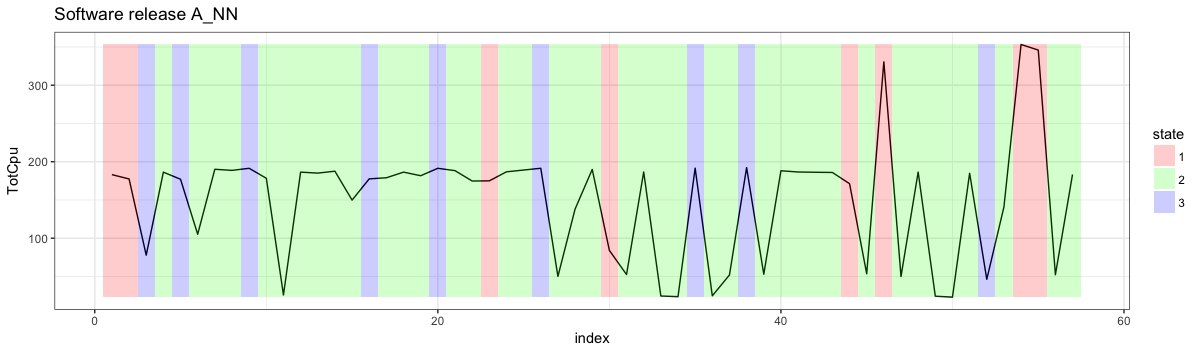
\includegraphics[scale=0.35]{picture/L16A_NN1}\caption{The CPU utilization of the software release A showing the periods
where the observation is in the specific state. \protect \\
Model 1: Fdd/Tdd and Numcells are non-switching coefficients.}
\label{L16A_NN}
\end{figure}


\subsection{Software release B}

For the software release B, \ref{L16B_switch} presents the results
of fitting the model with different combinations of switching coefficients.
Models 5 and 7 have higher BICs than the model which have switching
effects in all coefficients. The second model, where \emph{DuProdName}
and \emph{Fdd/Tdd} are non-switching coefficients, has the smallest
BIC. The chosen model for this dataset is the model which has only
\emph{DuProdName} as a non-switching coefficient or model 4.

\begin{table}[h]
\caption{List of the model structure of the software release B along with its
BIC. The last line is the result taken from the three-state model
in the Analysis I. The line in bold indicates the selected model.}
\label{L16B_switch}
\centering{}%
\begin{tabular}{ccccc}
\toprule 
\multirow{2}{*}{Model} & \multicolumn{3}{c}{Switching effect} & \multirow{2}{*}{BIC}\tabularnewline
\cmidrule{2-4} 
 & DuProdName & Fdd/Tdd & NumCells & \tabularnewline
\midrule
\midrule 
1 & N & N & N & 1787.528\tabularnewline
2 & N & N & Y & 1704.393\tabularnewline
3 & N & Y & N & 1784.384\tabularnewline
\textbf{4} & \textbf{N} & \textbf{Y} & \textbf{Y} & \textbf{1776.102}\tabularnewline
5 & Y & N & N & 1806.385\tabularnewline
6 & Y & N & Y & 1725.865\tabularnewline
7 & Y & Y & N & 1804.487\tabularnewline
\midrule
 & Y & Y & Y & 1797.259\tabularnewline
\bottomrule
\end{tabular}
\end{table}

Many switches between states can easily be seen in \ref{L16B_NYY}.
However, the state which has the longest duration remaining in its
own state is State3. There are three durations where the chain stays
in State3 for a long period of time. Another noticeable behavior from
this switching mechanism is that there are several switches to State1
and State2 in the beginning, middle, and at the end of the time period.
There are periods where the CPU utilization value does not change
much but the model identifies some switches. Also, there are periods
where the model fails to detect changes which is rather obvious.

\begin{figure}[H]
\begin{centering}
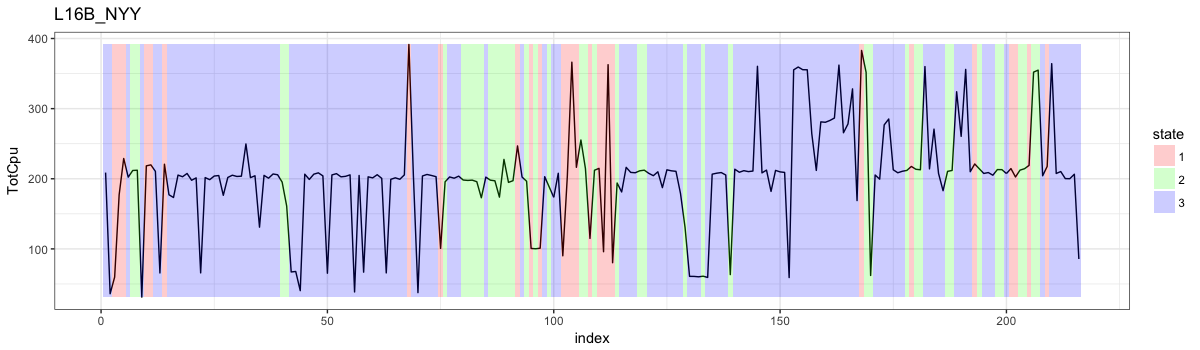
\includegraphics[scale=0.35]{picture/L16B_NYY1}
\par\end{centering}
\caption{The CPU utilization of the software release B showing the periods
where the observation is in the specific state. \protect \\
Model 4: DuProdName is non-switching coefficient.}
\label{L16B_NYY}
\end{figure}


\subsection{Software release C}

\ref{L17A_switch} presents model structure of the software release
C. Only model 2 has higher BIC than the model which have all switching
coefficients. The least BIC is from the first model of which all three
variables in the test environment have non-switching effects. This
model was also chosen to be further used for this dataset.

\begin{table}[h]
\caption{List of the model structure of the software release C along with its
BIC. The last line is the result taken from the three-state model
in the Analysis I. The line in bold indicates the selected model.}
\label{L17A_switch}
\centering{}%
\begin{tabular}{ccccc}
\toprule 
\multirow{2}{*}{Model} & \multicolumn{3}{c}{Switching effect} & \multirow{2}{*}{BIC}\tabularnewline
\cmidrule{2-4} 
 & DuProdName & Fdd/Tdd & NumCells & \tabularnewline
\midrule
\midrule 
\textbf{1} & \textbf{N} & \textbf{N} & \textbf{N} & \textbf{1140.474}\tabularnewline
2 & N & N & Y & 1204.280\tabularnewline
3 & N & Y & N & 1152.740\tabularnewline
4 & N & Y & Y & 1184.643\tabularnewline
5 & Y & N & N & 1146.000\tabularnewline
6 & Y & N & Y & 1189.236\tabularnewline
7 & Y & Y & N & 1157.311\tabularnewline
\midrule
 & Y & Y & Y & 1199.075\tabularnewline
\bottomrule
\end{tabular}
\end{table}

Several switches between three states occur in the beginning of the
time series as shown in \ref{L17A_NNN}. Around the end of the time
series period, State3 appears to have a longer duration and fewer
switches to State1. State2 seems to be the only state which has a
fairly short duration for the chain to stay in the state. Furthermore,
State2 tends to switch to State1 more often than to switch to State3.
The plot indicates some missed detections for this model which is
happened mostly in the durations of State3. 

\begin{figure}[H]
\begin{centering}
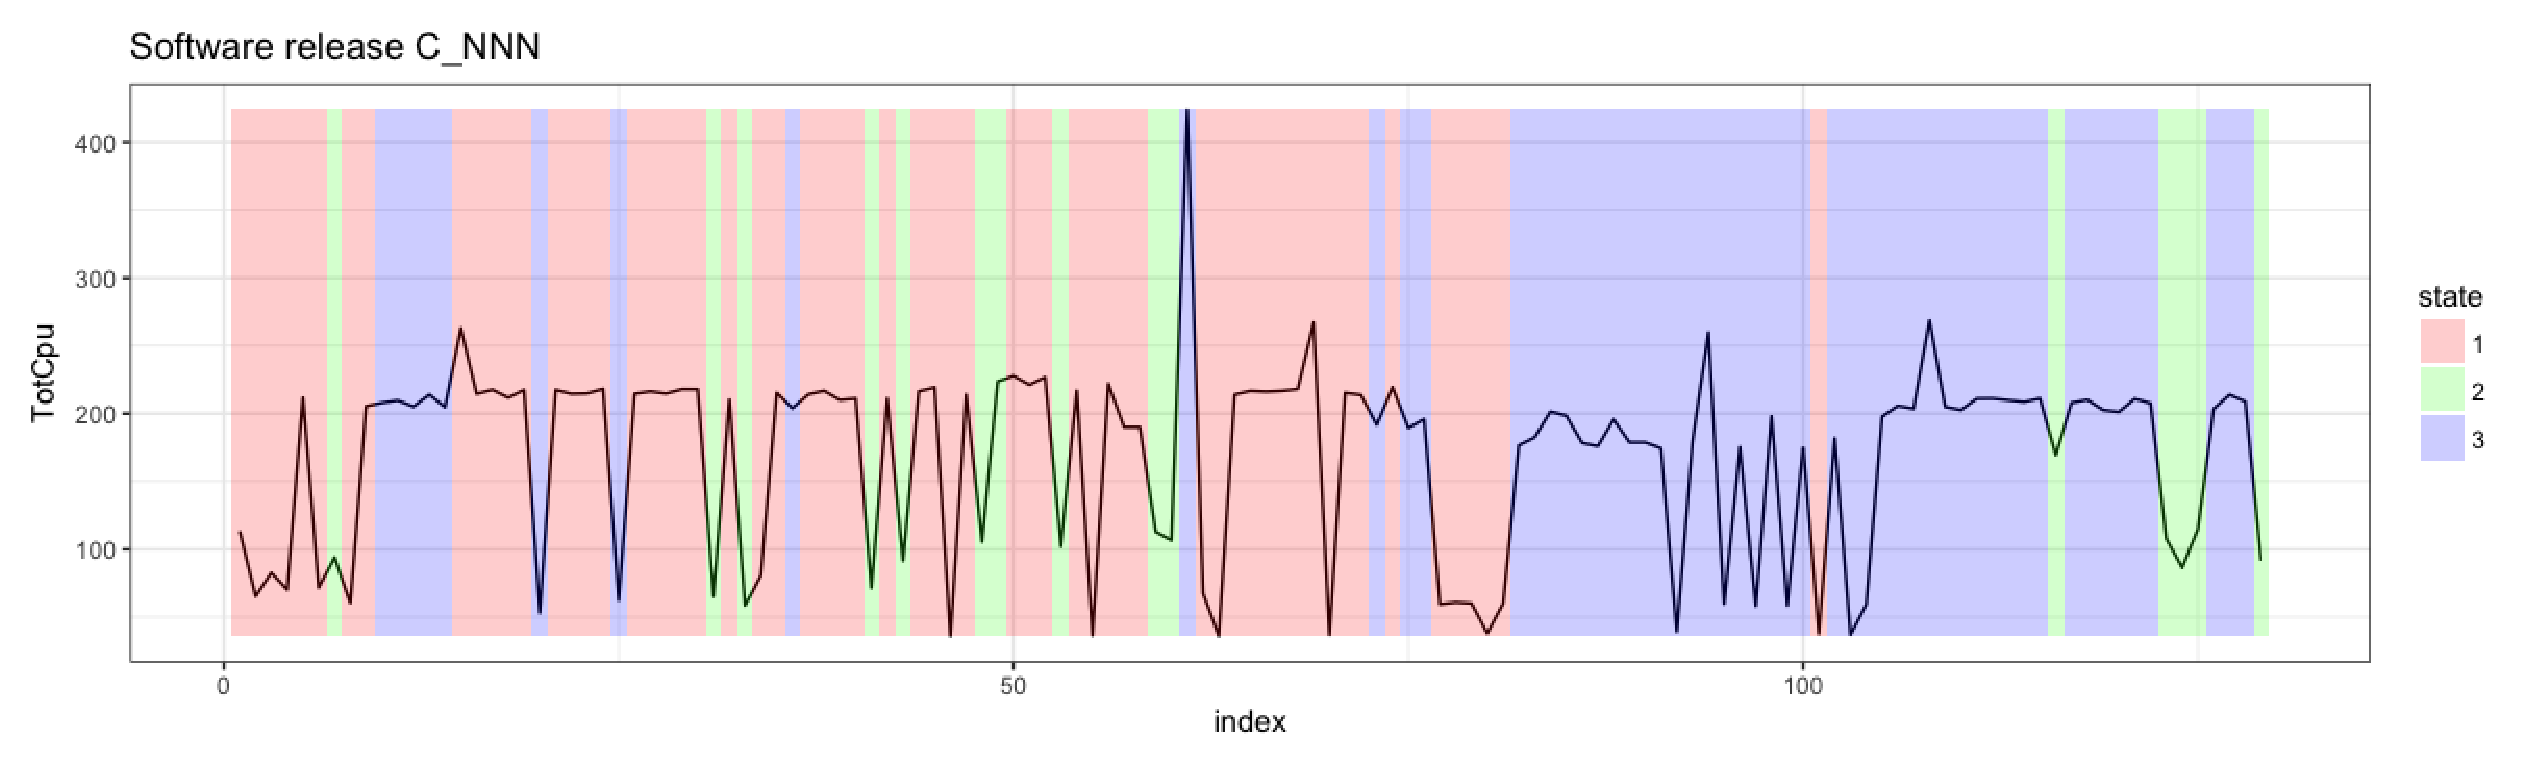
\includegraphics[scale=0.35]{picture/L17A_NNN1}
\par\end{centering}
\caption{The CPU utilization of the software release C showing the periods
where the observation is in the specific state. \protect \\
Model 1: DuProdName, Fdd/Tdd, and NumCells are non-switching coefficients.}
\label{L17A_NNN}
\end{figure}


\section{Residual analysis\label{sec:Residual}}

Pooled residuals of the selected Markov switching model from \ref{sec:Switching}
were analyzed to determine how well the model fitted with an assumption
of a normal distribution. A Quantile-Quantile (Q-Q) plot is an effective
tool for assessing normality. Moreover, an Autocorrelation function
(ACF) and a Partial Autocorrelation Function (PACF) of residuals are
a useful technique to check on the independence of noise terms in
the model. The Q-Q plot and the ACF/PACF plots play a significant
role in the residual diagnostics. These plots of each dataset are
shown in \ref{L16A_plotDiag}, \ref{L16B_plotDiag}, and \ref{L17A_plotDiag}. 

\subsection{Software release A}

In \ref{L16A_plotDiag}, the pooled residuals appear to fall in a
straight line with some deviations in its tails. There is an evidence
of autocorrelation in the residuals of this model, which can be seen
in both ACF and PACF plot, at lag 8. 

\begin{figure}[h]
\begin{centering}
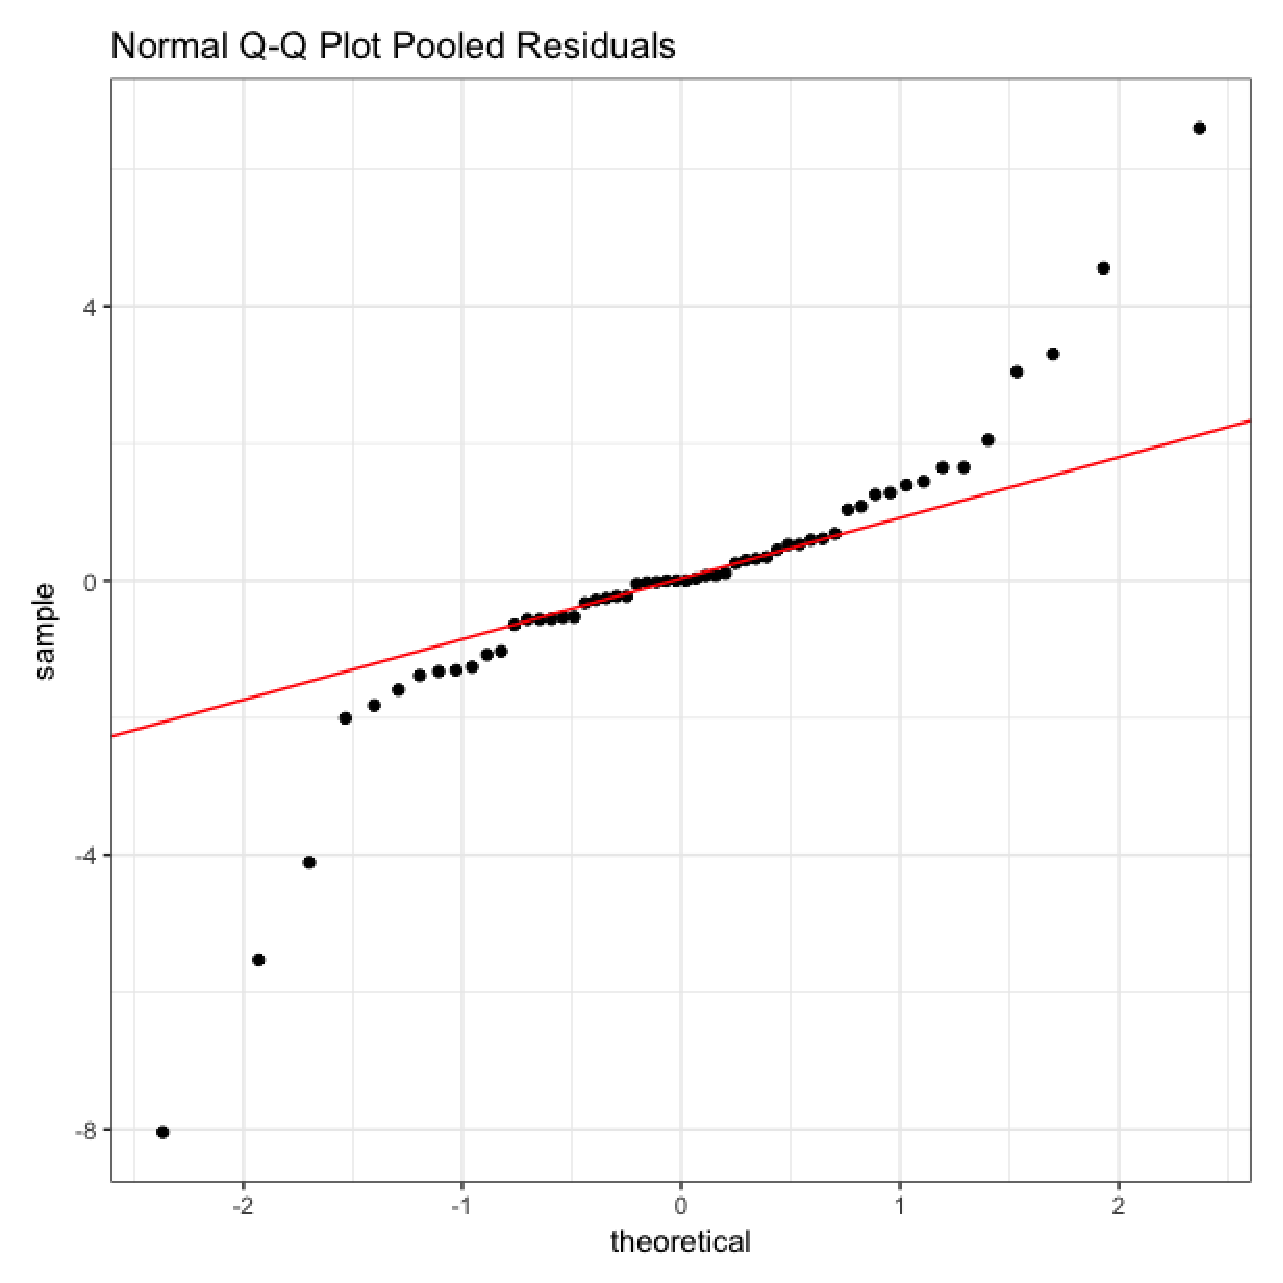
\includegraphics[scale=0.3]{picture/L16A_QQPool}$\quad$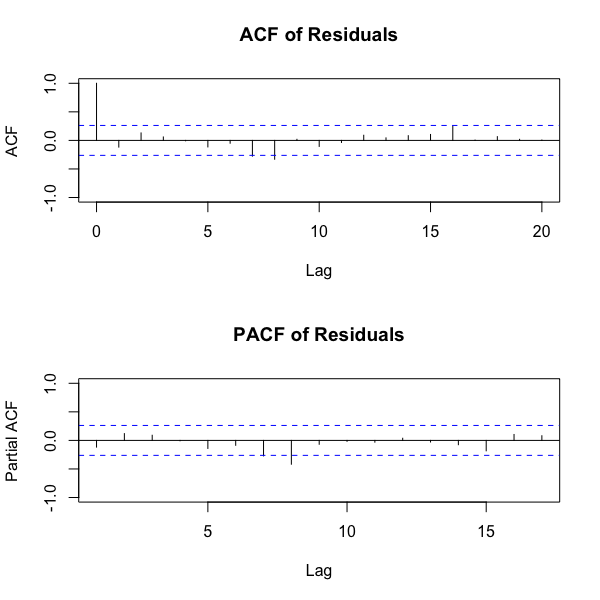
\includegraphics[scale=0.3]{picture/L16A_ACFPool}
\par\end{centering}
\caption{The normal Q-Q plot and the ACF/PACF of pooled residuals of the software
release A}
\label{L16A_plotDiag}
\end{figure}


\subsection{Software release B}

\ref{L16B_plotDiag} presents points that form a straight line in
the middle of the plot, but curve off at both ends. This is a characteristic
of a heavy-tailed distribution. The data has more extreme values than
it should if the data truly comes from a normal distribution. In addition,
both the ACF and PACF plots show that there is a small amount of autocorrelation
remaining in the residuals. The statistically significant correlation
of this model is at lags 6 and 10. The significance at lag 4 both
in the ACF and PACF plots is slightly higher than two standard errors.

\begin{figure}[H]
\begin{centering}
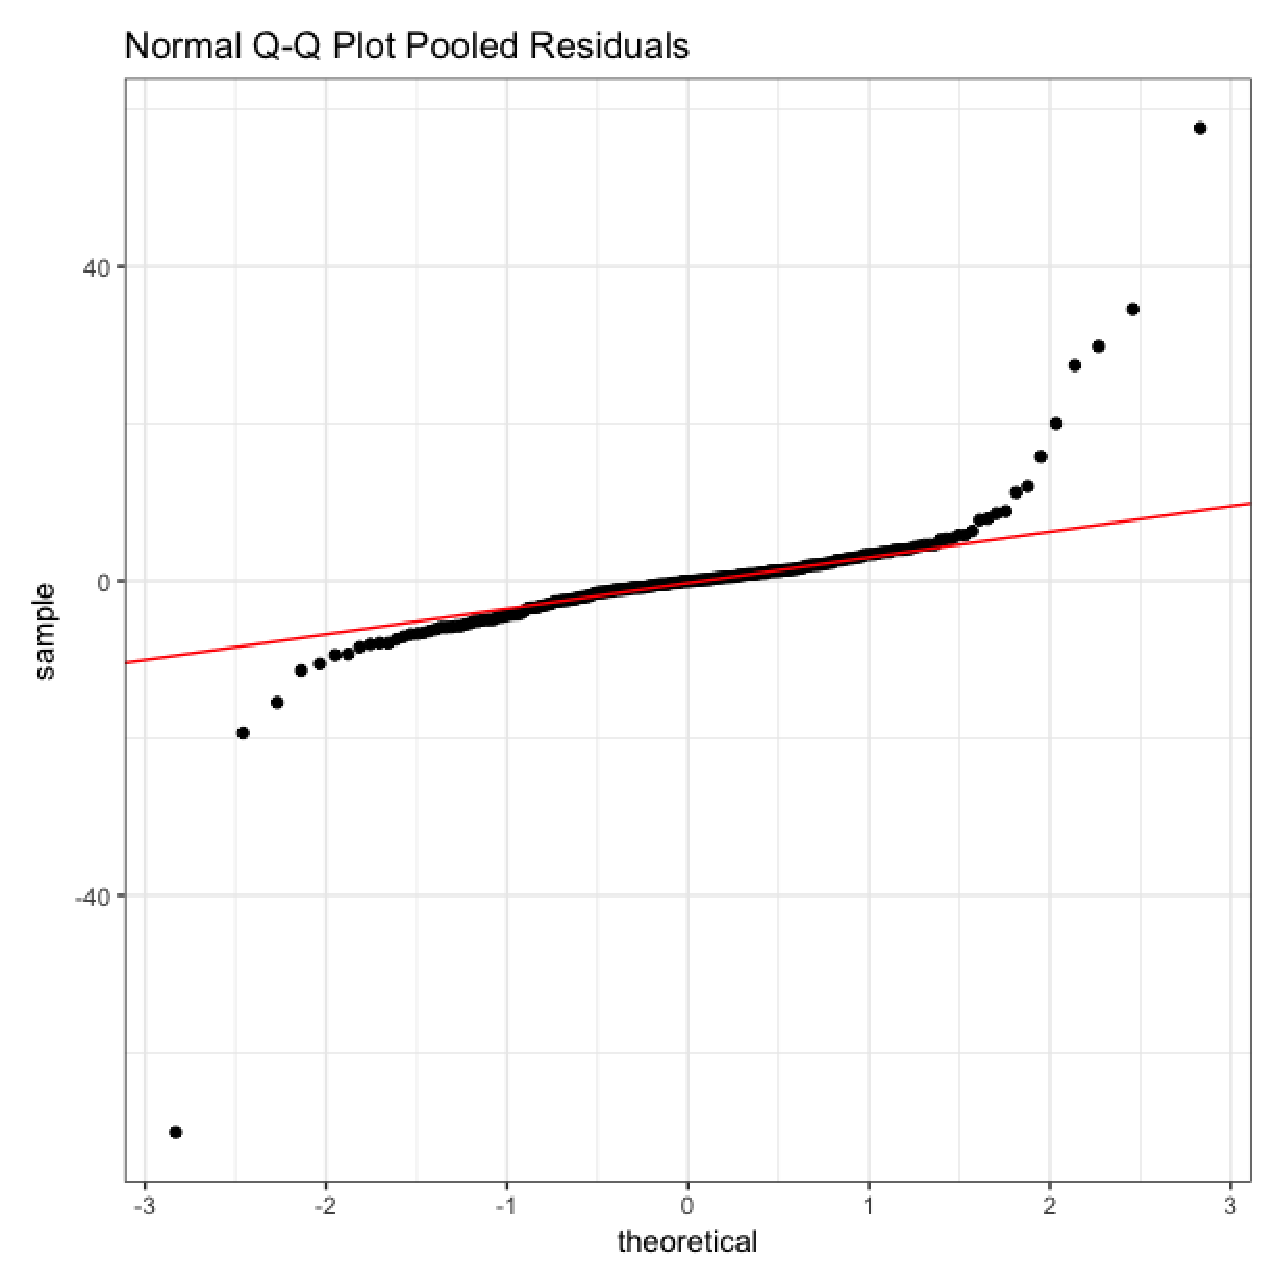
\includegraphics[scale=0.3]{picture/L16B_QQPool}$\quad$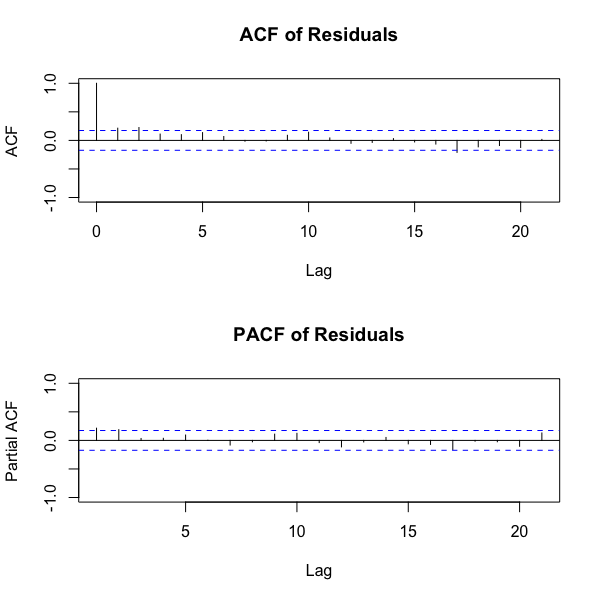
\includegraphics[scale=0.3]{picture/L16B_ACFPool}
\par\end{centering}
\caption{The normal Q-Q plot and the ACF/PACF of pooled residuals of the software
release B}
\label{L16B_plotDiag}
\end{figure}


\subsection{Software release C}

The Q-Q plot in \ref{L17A_plotDiag} suggests that a distribution
of the pooled residuals may have a tail thicker than that the one
of a normal distribution. It is visible that there are many extreme
positive and negative residuals in the plot. Furthermore, both the
ACF and PACF plots of pooled residuals are significant for the first
two lags. 

\begin{figure}[H]
\begin{centering}
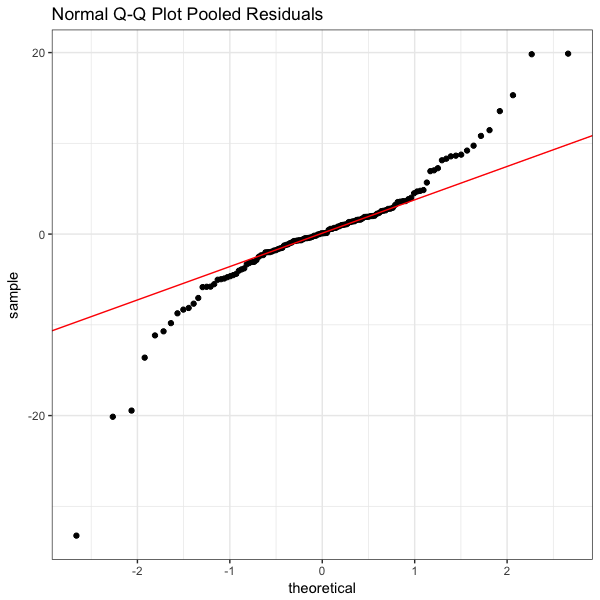
\includegraphics[scale=0.3]{picture/L17A_QQPool}$\quad$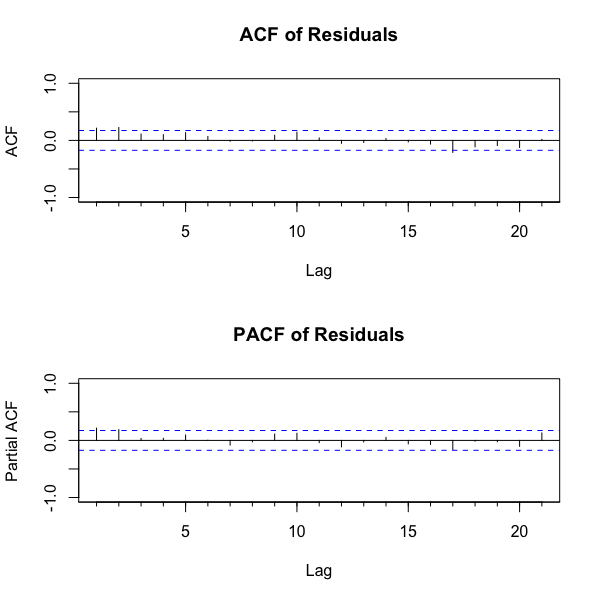
\includegraphics[scale=0.3]{picture/L17A_ACFPool}
\par\end{centering}
\caption{The normal Q-Q plot and the ACF/PACF of pooled residuals of the software
release C}
\label{L17A_plotDiag}
\end{figure}


\section{Non-parametric analysis}

An E-divisive method was applied to all three datasets. The method
reported one cluster for the dataset of the software release A and
five clusters for the dataset of each software release B and C. \ref{ediv}
shows places in the time series data where the E-divisive method detected
the significant changes. There is no estimated change point location
for the dataset of the software release A.

\begin{table}[h]
\caption{The locations of the statistically significant change points from
applying the E-divisive algorithm in each dataset}
\label{ediv}
\centering{}%
\begin{tabular}{cl}
\toprule 
Software release & Change-point location\tabularnewline
\midrule
\midrule 
A & -\tabularnewline
B & 130, 135, 153, 170\tabularnewline
C & 9, 77, 82, 105\tabularnewline
\bottomrule
\end{tabular}
\end{table}

The CPU utilization of the software release A, B and C along with
its estimated change points in the time series are plotted and shown
later in \ref{subsec:Real-data}. 

\section{Comparison between the Markov switching model and the E-divisive
method}

A comparison between the Markov switching model and the E-divisive
method was made in this section. These two methods were applied to
two simulated datasets, where the actual changes are already known
beforehand, and then also applied to a real data.

\subsection{Simulated Dataset 1}

\ref{compare_sim1} illustrates that the simulated data contains nine
estimated change point locations. For the Markov switching model,
the model reported two extra locations. The plot illustrates that,
besides the extra detected, the model performs rather well, as the
model discovers all the changes accurately. Only one change point
location was indicated to occur later than its actual occurrence time.
In contrast, the E-divisive method detected fewer changes than the
number of actual changes in the data. Furthermore, most of the detection
are also not quite accurate as three out of six detections are delayed
and one out of six detections is indicated to happen prior to its
actual time. The E-divisive method is unable to detect any changes
in the data at the beginning of the time period.

When these two methods detect changes after the actual changes, most
of their estimated change point locations are only behind by one or
two time index. To sum up, from this dataset, the Markov switching
model had more false alarms while the E-divisive had more missed detections. 

\begin{figure}[h]
\begin{centering}
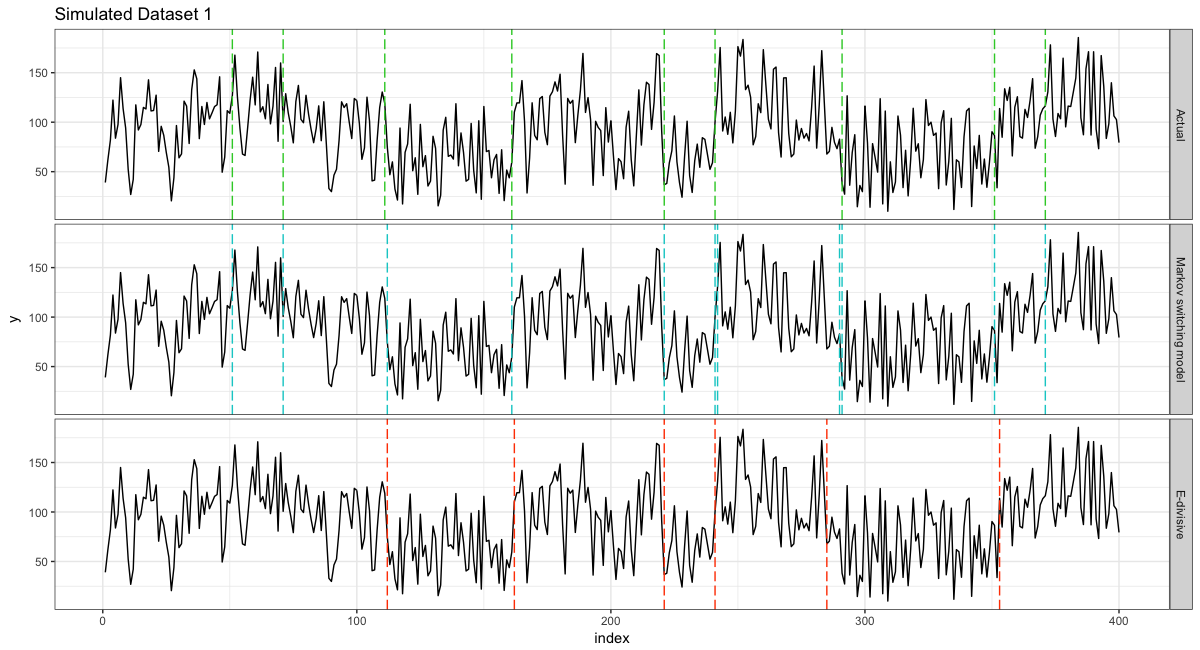
\includegraphics[scale=0.35]{picture/compare_sim1}
\par\end{centering}
\caption{The simulated Dataset 1 showing the estimated change point locations
indicated by dashed vertical lines from the Markov switching model
(Middle) and the E-divisive method (Bottom). The actual change point
locations in the data are indicated in the top plot. }

\label{compare_sim1}
\end{figure}


\subsection{Simulated Dataset 2}

\ref{compare_sim2} presents estimated change point locations of the
Markov switching model, the E-divisive method, and the actual change
points in the data. The simulated dataset contains numerous switches
between states. Generally, the Markov switching model is able to identify
the changes considerably well despite a few false alarms and missed
detections. On the other hand, the E-divisive method can detect only
two estimated change points. Both two detections were correctly located.
The method has quite poor performance as it failed to detect most
of the change points in the data. The difference can be seen in the
plot.

\begin{figure}[H]
\begin{centering}
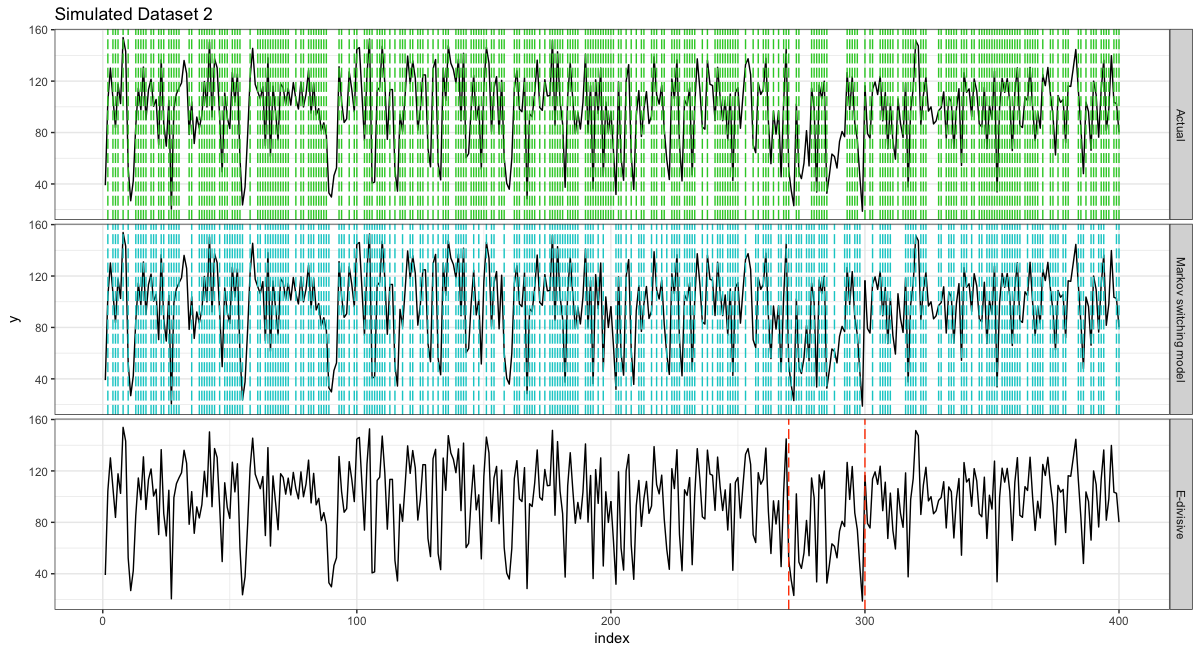
\includegraphics[scale=0.35]{picture/compare_sim2}
\par\end{centering}
\caption{The simulated Dataset 2 showing the estimated change point locations
indicated by dashed vertical lines from the Markov switching model
(Middle) and the E-divisive method (Bottom). The actual change point
locations in the data are indicated in the top plot. }

\label{compare_sim2}
\end{figure}


\subsection{Real data \label{subsec:Real-data}}

\subsubsection{Software release A}

According to \ref{ediv}, the E-divisive method could not identify
any changes in the dataset of the software release A. Thus, a comparison
between two methods could not be made for this dataset. 

\begin{figure}[H]
\begin{centering}
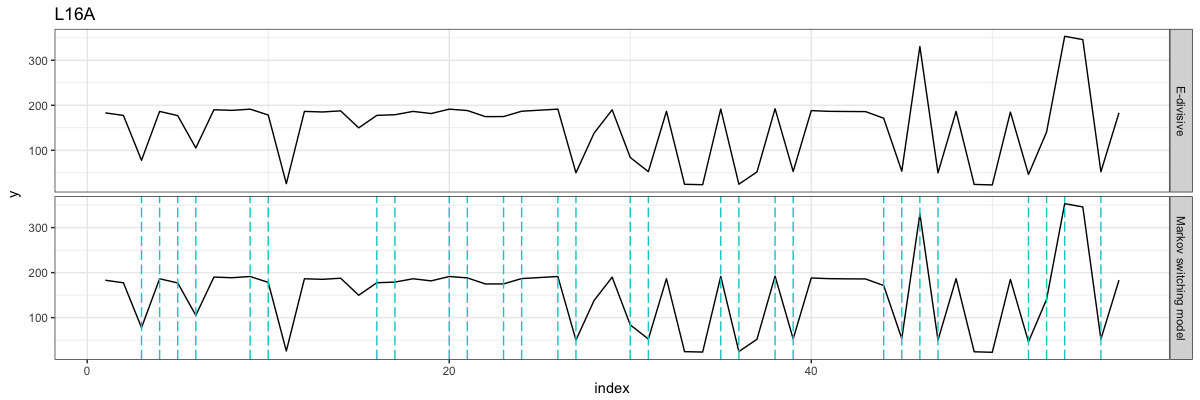
\includegraphics[scale=0.35]{picture/compare_L16A}
\par\end{centering}
\caption{The CPU utilization of the software release A. The dashed vertical
lines indicate the locations of estimated change points from the Markov
switching model (Top). }

\label{compare_L16A}
\end{figure}


\subsubsection{Software release B}

\ref{compare_L16B} presents results of estimated change points from
the Markov switching model and the E-divisive method for the software
release B. Sixty-three estimated change point locations are found
by the Markov switching model. On the contrary, only four estimated
change point locations are identified from the E-divisive method.
They are likely to occur around the same period of time. Most of the
locations of the change point detected by the E-divisive method are
at positive and negative peaks. Apparently, only one change point
location is determined at the exact same time from both methods, and
two change points are closely located. The rest of the detected locations
are completely different for each method.

\begin{figure}[H]
\begin{centering}
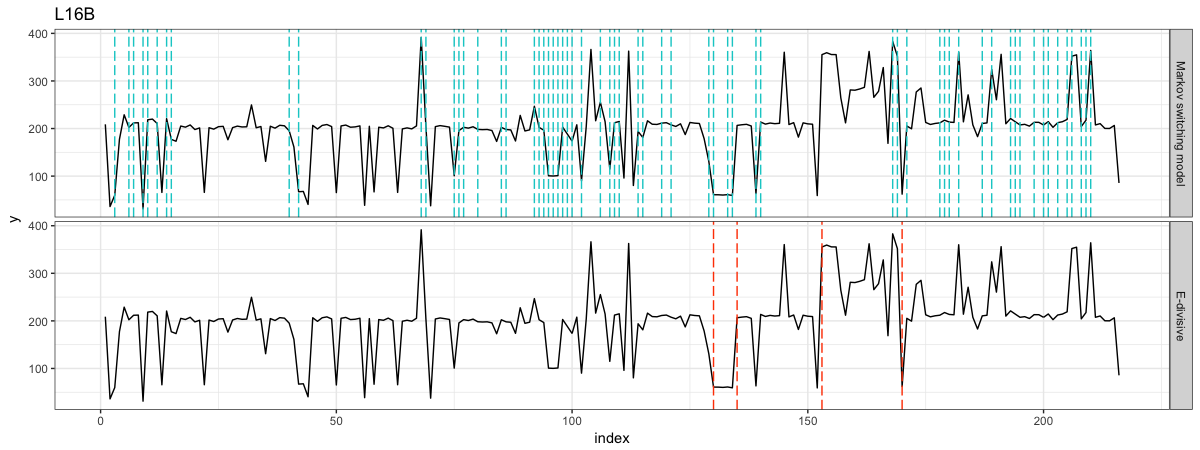
\includegraphics[scale=0.35]{picture/compare_L16B}
\par\end{centering}
\caption{The CPU utilization of the software release B. The dashed vertical
lines indicate the locations of estimated change points from the Markov
switching model (Top) and the E-divisive method (Bottom). }

\label{compare_L16B}
\end{figure}


\subsubsection{Software release C}

For the software release C, thirty-seven changes were discovered by
the Markov switching model as can be seen in \ref{compare_L17A}.
However, only four change point locations were identified from the
E-divisive method. These locations are rather spread out if compared
to the results from the software release B. The E-divisive method
discovered changes when the CPU utilization value was about to decrease
or increase. From both methods, two change points are determined at
exactly the same locations, and another one which is located in the
beginning is close to one another. Other detect locations are totally
different as shown in the plot. 

\begin{figure}[H]
\begin{centering}
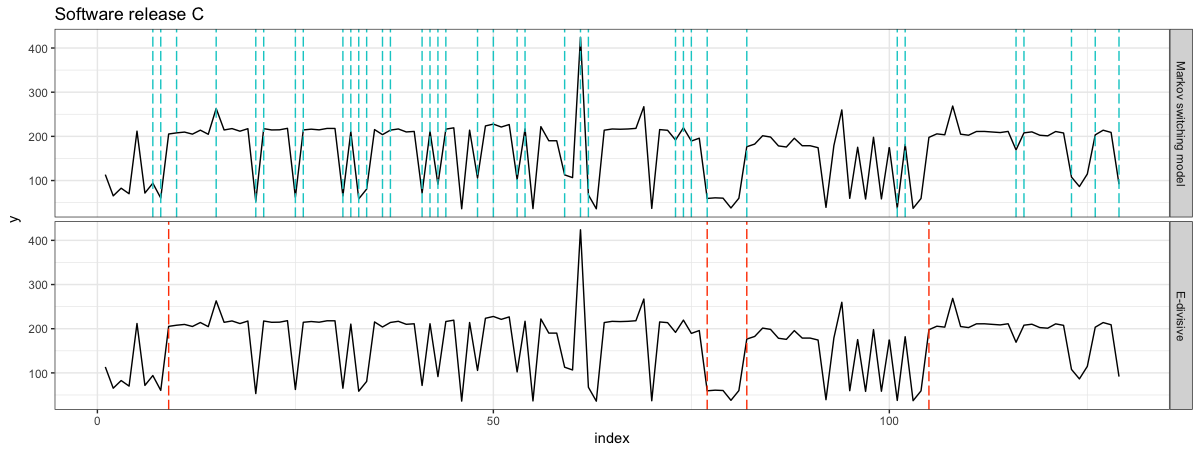
\includegraphics[scale=0.35]{picture/compare_L17A}
\par\end{centering}
\caption{The CPU utilization of the software release C. The dashed vertical
lines indicate the locations of estimated change points from the Markov
switching model (Top) and the E-divisive method (Bottom). }

\label{compare_L17A}
\end{figure}


\section{Predicting the state of the CPU utilization \label{sec:Predict}}

In this section, the state prediction function was implemented to
the test set in order to predict the most probable state for new observations. 

\subsection{Software release A}

For the software release A, there are 7 observations in total. In
\ref{predict_L16A}, only two states, State1 and State2, are assigned
for these observations. The first three observations are in State2.
Afterwards, the observations tend to switch back and forth between
both states until the end of the time period. Note that the most likely
state for the last observation of the test set is unable to be predicted,
and so it does not belong to any state.

\begin{figure}[h]
\begin{centering}
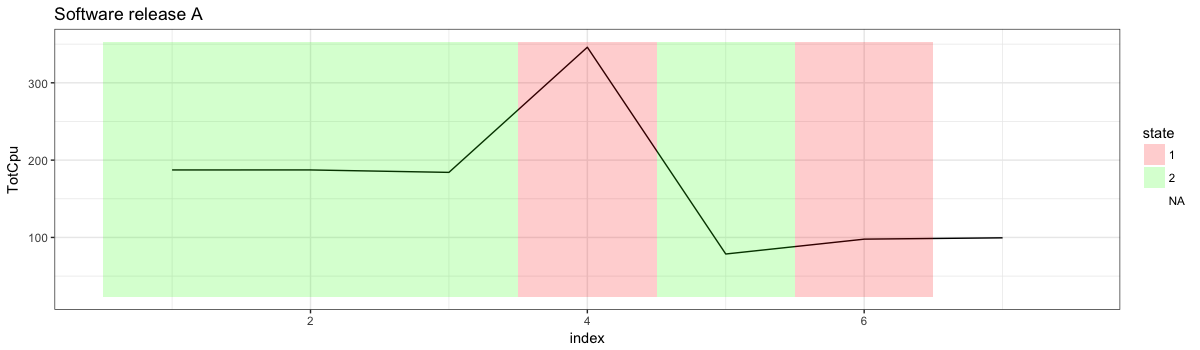
\includegraphics[scale=0.35]{picture/predict_L16A1}
\par\end{centering}
\caption{The predicted state of the test set in the software release A }

\label{predict_L16A}
\end{figure}


\subsection{Software release B}

In total, there are 25 observations in the test set of the software
release B. The result after applying the predict function to the test
set is shown in \ref{predict_L16B}. Observation 15 is the only observation
which is in State2. Many switches between State1 and State2 can be
seen from the plot. In addition, observation appears to stay in State1
only a short time before moving to State3, except for the first five
observations. 

\begin{figure}[h]
\begin{centering}
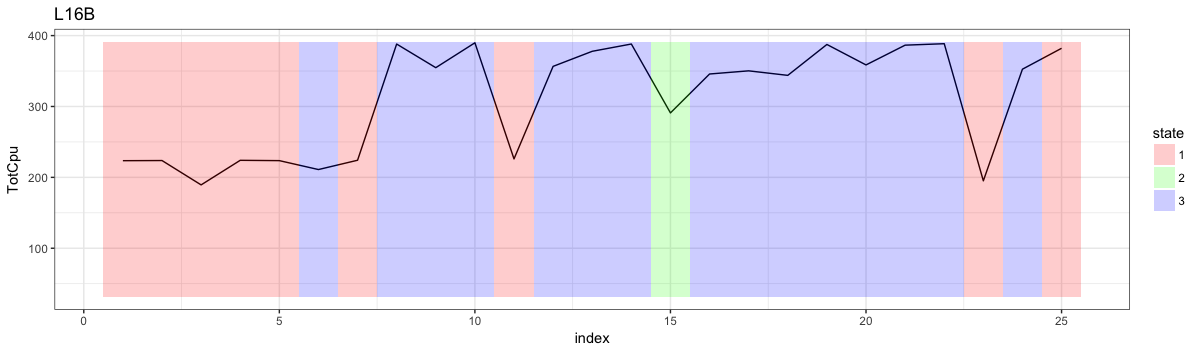
\includegraphics[scale=0.35]{picture/predict_L16B1}
\par\end{centering}
\caption{The predicted state of the test set in the software release B}

\label{predict_L16B}
\end{figure}


\subsection{Software release C}

The test set of the software release C consists of 15 observations
in total. \ref{predict_L17A} illustrates that the observations stay
in State2 for a considerably long period of time (observation 10-15).
There are several switches between states shown in the plot. The time
period between the observations between 4 and 7 switch between states
rapidly. The observations visit a particular state for one time, and
then immediately move to the another state. 

\begin{figure}[h]
\begin{centering}
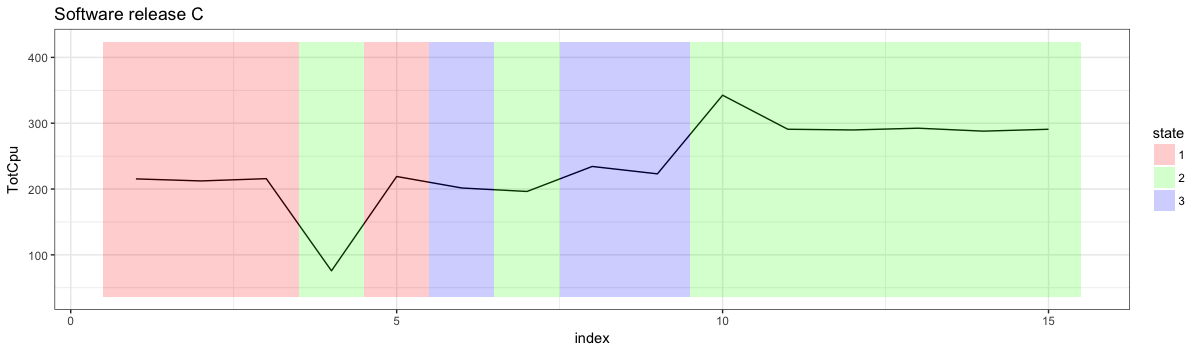
\includegraphics[scale=0.35]{picture/predict_L17A1}
\par\end{centering}
\caption{The predicted state of the test set in the software release C}
\label{predict_L17A}
\end{figure}


\section{Model evaluation \label{sec:Assessing}}

Eighty percents of the observations from the simulated data were fitted
with Markov switching model, and the remaining was used as a test
set to evaluate the performance of the model. 

\subsection{Simulated Dataset 1}

\ref{output-sim1} presents outputs from applying the Markov switching
model with the simulated Dataset 1. Each state has a considerably
high r-squared value which is greater than 0.9. From the results,
State2 has the highest standard error. When inferring back to the
actual models that were used to generate these three states in \ref{sec:Simulation},
it could be concluded that the result State1, State2, and State3 in
the table are a \emph{Bad}, \emph{Normal}, and \emph{Good} state,
respectively.

\begin{table}[H]
\caption{Outputs from applying the Markov switching model with the simulated
Dataset 1. The table shows estimated coefficients, residual standard
error, and r-squared for each state. A switching coefficient is followed
by (S), and a significant coefficient is highlighted in bold.}

\begin{centering}
\begin{tabular}{lr@{\extracolsep{0pt}.}lr@{\extracolsep{0pt}.}lr@{\extracolsep{0pt}.}l}
\toprule 
Estimated coefficient & \multicolumn{2}{c}{State 1} & \multicolumn{2}{c}{State 2} & \multicolumn{2}{c}{State 3}\tabularnewline
\midrule
\midrule 
(Intercept)(S) & \textbf{1}&\textbf{3024} & \textbf{5}&\textbf{5339} & \textbf{-14}&\textbf{3116}\tabularnewline
x1(S) & \textbf{0}&\textbf{8005} & \textbf{0}&\textbf{5900} & \textbf{0}&\textbf{7005}\tabularnewline
x2(S) & 0&0003 & \textbf{-0}&\textbf{8610} & \textbf{0}&\textbf{1941}\tabularnewline
y\_1(S) & \textbf{0}&\textbf{1902} & \textbf{0}&\textbf{3843} & \textbf{-0}&\textbf{1927}\tabularnewline
\midrule 
Residual standard error & 1&4900 & 7&3013 & 1&8255\tabularnewline
$r^{2}$ & 0&9980 & 0&9467 & 0&9962\tabularnewline
\bottomrule
\end{tabular}
\par\end{centering}
\centering{}\label{output-sim1}
\end{table}

The result of the model performance using Dataset 1 is shown in \ref{confusion}.
There are two observations from a \emph{Bad} state which were incorrectly
predicted to be in a Normal state. Moreover, two more observations
from a \emph{Good} state were predicted to be in a \emph{Normal} state.
The overall accuracy of the model is 0.96, and the misclassification
rate is 0.04. One can see that the model was able to perfectly predict
the state of the observations that are in a \emph{Normal} state. 

\begin{table}[h]
\caption{The confusion matrix of the result from the test set of the simulated
Dataset 1}
\label{confusion}
\centering{}%
\begin{tabular}{ccccc}
 & \multirow{1}{*}{} & \multicolumn{3}{c}{Predicted state}\tabularnewline
\cmidrule{2-5} 
 &  & Bad & Normal & Good\tabularnewline
\cmidrule{2-5} 
\multirow{3}{*}{Actual state} & Bad & 58 & 2 & 0\tabularnewline
\cmidrule{2-5} 
 & Normal & 0 & 30 & 0\tabularnewline
\cmidrule{2-5} 
 & Good & 0 & 2 & 8\tabularnewline
\cmidrule{2-5} 
\end{tabular}
\end{table}


\subsection{Simulated Dataset 2}

Outputs after applying the Markov switching model with the simulated
Dataset 2 are presented in \ref{output-sim2}. The r-squared values
of State1 and State3 are slightly lower than the obtained results
from the simulated Dataset 1, but the standard errors are significantly
higher. However, State2 has close output value to the simulated Dataset1.
It could be said that the model still performs rather well as the
r-squared value is very high. State1 is said to be a \emph{Bad} state
although an intercept is insignificant. State2 and State3 are a \emph{Good}
and \emph{Normal} state, respectively.

\begin{table}[H]
\caption{Outputs from applying the Markov switching model with the simulated
Dataset 2. The table shows estimated coefficients, residual standard
error, and r-squared for each state. A switching coefficient is followed
by (S), and a significant coefficient is highlighted in bold.}

\begin{centering}
\begin{tabular}{lr@{\extracolsep{0pt}.}lr@{\extracolsep{0pt}.}lr@{\extracolsep{0pt}.}l}
\toprule 
Estimated coefficient & \multicolumn{2}{c}{State 1} & \multicolumn{2}{c}{State 2} & \multicolumn{2}{c}{State 3}\tabularnewline
\midrule
\midrule 
(Intercept)(S) & 5&0716 & \textbf{9}&\textbf{0219} & \textbf{23}&\textbf{1711}\tabularnewline
x1(S) & \textbf{0}&\textbf{8672} & \textbf{0}&\textbf{5401} & \textbf{0}&\textbf{5546}\tabularnewline
x2(S) & -0&0195 & \textbf{0}&\textbf{2599} & \textbf{-1}&\textbf{1239}\tabularnewline
y\_1(S) & \textbf{0}&\textbf{1232} & \textbf{-0}&\textbf{0882} & \textbf{0}&\textbf{2272}\tabularnewline
\midrule 
Residual standard error & 6&6367 & 5&3211 & 7&5079\tabularnewline
$r^{2}$ & 0&9089 & 0&9480 & 0&9337\tabularnewline
\bottomrule
\end{tabular}
\par\end{centering}
\centering{}\label{output-sim2}
\end{table}

\ref{confusion2} presents a confusion matrix for a test set from
a second simulated dataset. The model was able to correctly predict
all the observations in a \emph{Bad} state. On the contrary, the model
did not perform well in predicting observations which had \emph{Good}
state. Nine observations from a \emph{Good} state were predicted to
be in a \emph{Bad} state, and another five observations from a \emph{Good}
state were inaccurately predicted to be in a \emph{Norma}l state.
Six observations from a \emph{Normal} state were incorrectly predicted
to be in a \emph{Good} state. The overall accuracy of the model and
the misclassification rate are 0.8 and 0.2, respectively. 

\begin{table}[h]
\caption{The confusion matrix of the result from the test set of the simulated
Dataset 2}
\label{confusion2}
\centering{}%
\begin{tabular}{ccccc}
 & \multirow{1}{*}{} & \multicolumn{3}{c}{Predicted state}\tabularnewline
\cmidrule{2-5} 
 &  & Bad & Normal & Good\tabularnewline
\cmidrule{2-5} 
\multirow{3}{*}{Actual state} & Bad & 35 & 0 & 0\tabularnewline
\cmidrule{2-5} 
 & Normal & 0 & 29 & 6\tabularnewline
\cmidrule{2-5} 
 & Good & 9 & 5 & 16\tabularnewline
\cmidrule{2-5} 
\end{tabular}
\end{table}


